\documentclass[aps,prc,twocolumn,floatfix,preprintnumbers]{revtex4}
%\usepackage{hyperref}
\usepackage{graphicx}
\usepackage{amsmath}
\usepackage{amsfonts}
\usepackage{color}

\newcommand{\coral}{{\tt CorAL}}
\newcommand{\reefer}{{\tt reefer}}

%=============================================================================
%  Frontmatter
%=============================================================================
\begin{document}

\title{{\tt CorAL} User's Guide}

\preprint{\rm UCRL-MA-?????}

\author{David Brown}
\author{Mike Heffner}
\affiliation{Lawrence Livermore National Laboratory, Livermore, CA 94550 USA}

\date{\today}

\begin{abstract}
empty abstract
\end{abstract}

\maketitle
   
%=============================================================================
%  Main Text
%=============================================================================
\section{Introduction}
\coral\, rules!

We work in the Bertsch-Pratt coordinates in the pair center of mass frame.

\begin{figure}
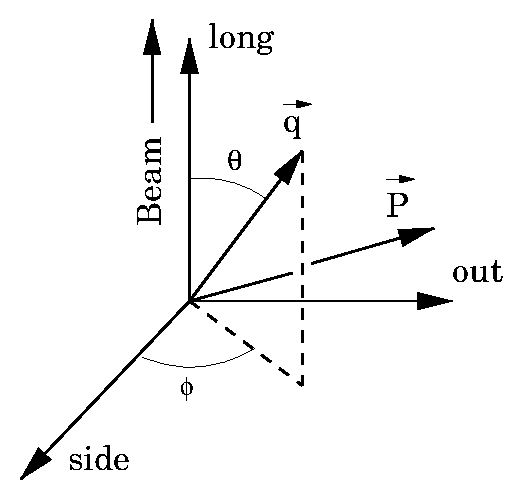
\includegraphics[width=0.4\textwidth]{coords}
\caption{The Bertsch-Pratt coordinates.}
\label{coords}
\end{figure}

\section{Global Parameters}
Global parameters are set upon creation of the globalparameters class, using the
following scheme:
\begin{enumerate}
    \item Check command line for name of user's global parameter file
    \item failing that, check for ``{\tt prefs.dat}''
    \item failing that, default to settings in constructor
\end{enumerate}

Table~\ref{globalparams} lists all of the global parameters used by the code.
You can put others in your prefs.dat file, but they will be ignored by the code.

The syntax for the file is as follows.  Each entry is put in like:\\
\verb+<option> = <setting>+

\begin{table*}
\begin{tabular}{|c|c|c|}
    \hline
    Option                 & Default Value & Description\\ \hline
    {\tt messaging\_level} & 0             & description\\ \hline
    {\tt momentum\_units}  & MeV           & description\\ \hline
    {\tt distance\_units}  & fm            & description\\ \hline
    {\tt comment\_string}  & \#            & description\\ \hline
\end{tabular}
\caption{Global settings.}
\label{globalparams}
\end{table*}


\section{Input Command File}

There is a front-end for \coral\, called \reefer.  \reefer\, takes a text file as 
input and attempts to carry out the commands listed in this file.  The commands
all have the following syntax:
\begin{verbatim}
<action> <input_string> <output_string> {
    [options]
}
\end{verbatim}
Note that the different tokens are separated by whitespace and any or all of a
line may be commented out with the comment string (by default this is set to
``\#'', but may be changed in the global preferences).  Here {\tt 
<input\_object>} and {\tt <output\_object>} are 
either {\tt Object}s, such as a correlations or a sources, or file names.  
Table~\ref{commands} is a complete list of commands and what things they act 
on.
\begin{table*}
\begin{tabular}{|c|c|c|l|}
    \hline\hline
    Command & First Argument  & Second Argument & Short Description\\ \hline\hline
    \multicolumn{4}{|l|}{\bf Input/Output Commands}\\ \hline
    {\tt read} & object name & file name  & Reads {\tt Object} from file \\ \hline
    {\tt write} & object name & file name & Writes {\tt Object} to file\\ \hline
    {\tt create} & object name & object type & Creates an {\tt Object}\\ \hline
    \multicolumn{4}{|l|}{\bf Correlation/Source Processing Commands}\\ \hline
    {\tt expand} & name of a {\tt corr\_3d\_cart} & name of a {\tt corr\_3d\_sphr} & Expands correlation in $Y_{\ell m}$'s\\ \hline
    {\tt unexpand} & name of a {\tt corr\_3d\_sphr} &  name of a {\tt corr\_3d\_cart}  & Converts a correlation from spherical to cartesian coords.\\
                   &                                &                                  & (inverse of {\tt expand})\\ \hline
    {\tt image} & name of a correlation & name of a source & Images a correlation\\ \hline
    {\tt unimage} & name of a source & name of a correlation & Reconstructs correlation from imaged source\\ 
                  &                  &                       & (inverse of {\tt image})\\ \hline
    \multicolumn{4}{|l|}{\bf Commands for Characterizing Correlation/Sources}\\ \hline
    {\tt gaussparam} & name of a source  & n/a & Does a cheezy ``fit'' to a Gaussian\\ \hline
    {\tt intbump} & object name & n/a & Integrates the volume under the bump of a corr or source\\ \hline
    {\tt powspec} & name of a {\tt corr\_3d\_sphr} & n/a & Computes power spectrum of source as function of $\ell$\\ \hline
    \multicolumn{4}{|l|}{\bf Plotting Commands}\\ \hline
    {\tt slicerad} & object name & file name & description\\ \hline
    {\tt slices} & object name & file name & description\\ \hline
    {\tt sliceo} & object name & file name & description\\ \hline
    {\tt slicel} & object name & file name & description\\ \hline
    {\tt sliceso} & object name & file name & description\\ \hline
    {\tt slicesl} & object name & file name & description\\ \hline
    {\tt sliceol} & object name & file name & description\\ \hline
    \multicolumn{4}{|l|}{\bf Misc. Commands}\\ \hline
    {\tt stop} & n/a & n/a & Stops script execution and exits program\\ \hline
    {\tt exit} & n/a & n/a & Alias for {\tt stop}\\ \hline
    {\tt quit} & n/a & n/a & Alias for {\tt stop}\\ \hline
    {\tt list} & n/a & n/a & Lists all objects in the Object Registry\\ \hline
    {\tt help} & n/a & n/a & Lists all of the {\tt reefer} commands\\ \hline
    {\tt help} & command name & n/a & Help for specific command\\ \hline
    {\tt delete} & object name & n/a & Deletes object from Object Registry\\ \hline
    {\tt setprefix} & object name  & new prefix & Renames the file prefix of all terms in a 3d object\\ \hline
    {\tt rename} & old object name & new object name  & Renames an object\\ \hline
    {\tt typeof} & object name & n/a  & Prints type of object\\ \hline
    {\tt print} & object name & n/a  & Prints object\\ \hline
    {\tt import} & file name & n/a & imports and processes {\tt file name} \\ \hline
    {\tt preferences} & n/a & n/a  & Prints global preferences\\ \hline
    \multicolumn{4}{|l|}{\bf Unimplemented Commands}\\ \hline
    {\tt copy} & object name 1 & object name 2 & Copies object 1 to 2\\ \hline
    {\tt copyterm} & object name 1 & object name 2 & Copies on term of object 1 to 2\\ \hline
    {\tt cd} & directory & n/a  & Changes working directory\\ \hline
    {\tt fit} & ?? & ?? & unimplemented\\ \hline
    {\tt fixtail} & name of a correlation & n/a & unimplemented\\ \hline
    {\tt chi2} & name of a correlation & name of a correlation & unimplemented\\ \hline
    {\tt boost} & object name & n/a & unimplemented\\ \hline
    {\tt } &  &  & description\\ \hline\hline
\end{tabular}
\caption{\reefer\, commands.}
\label{commands}
\end{table*}

\begin{table*}
\begin{tabular}{|c|c|c|c|}
    \hline\hline
    Object  & Short Description\\ \hline\hline
    \multicolumn{2}{|l|}{\bf Source Functions}\\ \hline
    {\tt source\_1d\_term}  &description\\ \hline
    {\tt source\_3d\_sphr} &  description\\ \hline
    {\tt source\_1d\_gaussian} &  description\\ \hline
    {\tt source\_1d\_2gaussian} &  description\\ \hline
    {\tt source\_1d\_blastwave} &  description\\ \hline
    {\tt source\_3d\_gaussian} &  description\\ \hline
    {\tt source\_3d\_blastwave} &  description\\ \hline
    {\tt source\_1d\_crab} &  description\\ \hline
    {\tt source\_3d\_crab} &  description\\ \hline
    \multicolumn{2}{|l|}{\bf Correlation Functions}\\ \hline
    {\tt corr\_1d\_term} &  description\\ \hline
    {\tt corr\_3d\_cart} &   description\\ \hline
    {\tt corr\_3d\_sphr} &   description\\ \hline
    \multicolumn{2}{|l|}{\bf Emission Functions}\\ \hline
    {\tt emissfunc\_blastwave}& description\\ \hline
    {\tt } &  description\\ \hline\hline
\end{tabular}
\caption{\reefer\, objects.}
\label{objects}
\end{table*}

When a new object is created, \coral\, attempts to create it with reasonable
defaults.  When a \reefer\, command is executed, \reefer\, uses these defaults
unless overidden in the input file.  To control the way a new object is made, 
add a section after a command as follows:
\begin{verbatim}
<action> <input_string> <output_string>{
    [option 1] = <value 1>
    [option 2] = <value 2>
    .
    .
    .
    <datablock> {
        <data in columns>
        .
        .
        .
        
    }
    <string_list> {
        <string>
        .
        .
        .
        
    }
}
\end{verbatim}

{\tt Object}s are also described in this manner, but with a few additions.  
The main difference being that {\tt Object} descriptions may have nested
sections:
\begin{verbatim}
<object> {
    [option 1] = <value 1>
    [option 2] = <value 2>
    .
    .
    .
    <datablock> {
        <data in columns>
        .
        .
        .
        
    }
    <string_list> {
        <string>
        .
        .
        .
        
    }
    .
    .
    .
}
\end{verbatim}
The purpose of such subsections is to store the actual data of the object.  They
are described in each {\tt object}'s description.


\section{Command Options}
In this section, we list all of the options available to each command and the
defaults.

\subsection{{\tt read}}
Reads in an {\tt Object} named {\tt <object\_name>} from file {\tt
<file\_name>} and inserts it into the {\tt ObjectMap}.  It is invoked by:
\begin{verbatim}
read <object_name> <file_name>
\end{verbatim}

\subsection{{\tt write}}
Writes an {\tt Object} named {\tt <object\_name>} from the {\tt ObjectMap} to 
file {\tt <file\_name>}.  It is invoked by:
\begin{verbatim}
write <object_name> <file_name>
\end{verbatim}

\subsection{{\tt create}}
\begin{verbatim}
create <object_name> <object_type>
\end{verbatim}

\subsection{{\tt expand}}
\begin{verbatim}
expand <3d_cart corr name> <3d_sphr corr name>
\end{verbatim}

\subsection{{\tt unexpand}}
\begin{verbatim}
unexpand <3d_sphr corr name> <3d_cart corr name>
\end{verbatim}

\subsection{{\tt image}}
\begin{verbatim}
image <corr_name> <source_name>
\end{verbatim}

\subsection{{\tt unimage}}
\begin{verbatim}
unimage <source_name> <corr_name>
\end{verbatim}

\subsection{{\tt chi2}}
\begin{verbatim}
chi2 <corr1>  <corr2> 
\end{verbatim}

\subsection{{\tt gaussparam}}
\begin{verbatim}
gaussparam <source_name> 
\end{verbatim}

\subsection{{\tt intbump}}
\begin{verbatim}
intbump <object_name>
\end{verbatim}

\subsection{{\tt powpec}}
\begin{verbatim}
powspec <object_name> 
\end{verbatim}

\subsection{{\tt fit}}
\begin{verbatim}
fit <corr_name>
\end{verbatim}

\subsection{{\tt fixtail}}
\begin{verbatim}
fixtail <corr_name> 
\end{verbatim}

\subsection{{\tt list}}
\begin{verbatim}
list
\end{verbatim}

\subsection{{\tt delete}}
\begin{verbatim}
delete <object_name> 
\end{verbatim}

\subsection{{\tt rename}}
\begin{verbatim}
rename <old_name> <new_name> 
\end{verbatim}

\subsection{{\tt help}}
\begin{verbatim}
help
\end{verbatim}

\subsection{{\tt quit}, {\tt stop}, {\tt exit}}
\begin{verbatim}
stop
\end{verbatim}

\subsection{{\tt import}}
\begin{verbatim}
import <filename> 
\end{verbatim}

\subsection{{\tt cd}}
\begin{verbatim}
cd <directory> 
\end{verbatim}

\subsection{{\tt slicerad}}
Makes a file called {\tt <file\_name>} containing a slice of the object along
the angle $\theta=${\tt theta}, $\phi=${\tt phi} in the Bertsch-Pratt
coordinates.  Here $\theta$ is the angle with respect to the longitudinal axis
(the z-axis) and $\phi$ is the angle with respect to the sidewards axis (the
x-axis).  It is invoked by:
\begin{verbatim}
slicerad <object_name> <file_name> {
    theta = <angle in rad>
    phi = <angle in rad>
}
\end{verbatim}
The output from this command is a file which contains a few lines of header
information and 5 columns of data.  As is, the file can be plotted using the 
package {\tt xmgrace}.

\subsection{{\tt slices}, {\tt sliceo}, {\tt slicel}}

\subsection{{\tt sliceso}, {\tt slicesl}, {\tt sliceol}}



\section{Object Options}
In this section, we list all of the options available to each object and the
defaults.

\subsection{{\tt source\_1d\_term}}


\subsection{{\tt source\_3d\_sphr}}


\subsection{{\tt source\_1d\_gaussian}}


\subsection{{\tt source\_3d\_gaussian}}


\subsection{{\tt source\_1d\_crab}}


\subsection{{\tt source\_3d\_crab}}


\subsection{{\tt corr\_1d\_term}}


\subsection{{\tt corr\_3d\_cart}}


\subsection{{\tt corr\_3d\_sphr}}




\section{Kernels}


\acknowledgments
This work was performed under the auspices of the U.S. Department of Energy by University of California, Lawrence Livermore National Laboratory under Contract W-7405-Eng-48.

\appendix
\section{Extending Source and Correlation Classes}
\section{Source and Correlation Templates}

%=============================================================================
%  References
%=============================================================================
\onecolumngrid
\begin{thebibliography}{70}

  \bibitem{coderef} \coral\, Code Reference.

  \bibitem{testentry} testentry 

\end{thebibliography}

\end{document}
